\documentclass[12pt,a4paper,twoside]{report}

%%%%%%%%%%%%%%%%%%%%%%%%%%%%%%%%%%%%%%%%%%%%%%%%%%%%%%%%%%%%%%%%%%%%%%%%
%%%%%%%%%%%% Packages %%%%%%%%%%%%%%%%%%%%%%%%%%%%%%%%%%%%%%%%%%%%%%%%%%
%%%%%%%%%%%%%%%%%%%%%%%%%%%%%%%%%%%%%%%%%%%%%%%%%%%%%%%%%%%%%%%%%%%%%%%%

%%%%%%
% In general useful packages
%%%%%%
\usepackage[latin1]{inputenc} % allow Umlauts
\usepackage[T1]{fontenc} % Umlauts as character in font
\usepackage{fancyhdr}   % Header/Footer
\usepackage[pdftex]{graphicx}

%%%%%%
% The following packages are optional, uncomment them if useful and required
%%%%%%
\usepackage{fancyvrb}   % extended verbatim environment
% \usepackage{latexsym}   % additional symbols
% \usepackage{times}      % bessere Schrift in PS-Dateien
% \usepackage{longtable}  % long tables (with page breaks)
% \usepackage{breakcites}  % linebreaks in cites

\usepackage[us]{datetime} % date in \today as "Month DD, YYYY", e.g., "February 29, 2012"

%%%%%%
% Hyperlinks in PDF output (blue borders, text color unchanged)
%%%%%%
\usepackage[plainpages=false, pdfpagelabels, bookmarks,  colorlinks=false,
               linkbordercolor={0 0 1}, filebordercolor={0 0 1}, citebordercolor={0 0 1},
               menubordercolor={0 0 1}, pagebordercolor={0 0 1}, urlbordercolor={0 0 1}]{hyperref}

%%%%%%
% Another set of useful packages
%%%%%%
% \usepackage[square]{natbib}  % more powerful and customizable references
% \usepackage[center]{caption} % centered, multi-line captions of figures and tables
% \usepackage{floatflt}        % floats (e.g., figures & tables) which can have floating text around them
% \usepackage[thmmarks]{ntheorem}    % extended theorem environment
\usepackage{pdfcomment}  % comments in text as PDF notes

%%%%%%%%%%%%%%%%%%%%%%%%%%%%%%%%%%%%%%%%%%%%%%%%%%%%%%%%%%%%%%%%%%%%%%%%
%%%%%%%%%%%% Layout %%%%%%%%%%%%%%%%%%%%%%%%%%%%%%%%%%%%%%%%%%%%%%%%%%
%%%%%%%%%%%%%%%%%%%%%%%%%%%%%%%%%%%%%%%%%%%%%%%%%%%%%%%%%%%%%%%%%%%%%%%%
% German style (no paragraph indent, but gap between paragraphs)
% \setlength{\parindent}{0mm}
% \setlength{\parskip}{4pt plus3pt minus2pt}

% Page width and margins (usually no need to change, just use a4wide package)
% \setlength{\textwidth}{15cm}
% \addtolength{\oddsidemargin}{1mm}
% \addtolength{\evensidemargin}{-13.5mm}
\usepackage{a4wide} % better than individual setup

% For fancyhdr, otherwise it might result in "overfull vbox"
\addtolength{\headheight}{3.5pt}

% URL Prefix for Bibliography (i.e., no prefix, typewriter as font for URLs)
\newcommand{\urlprefix}{}
\def\UrlFont{\small\tt}
%\urlstyle{rm} % oder sf, falls obiges nicht funktioniert


%%%%%%%%%%%%%%%%%%%%%%%%%%%%%%%%%%%%%%%%%%%%%%%%%%%%%%%%%%%%%%%%%%%%%%%%
%%%%%%%%%%%% Some useful macros %%%%%%%%%%%%%%%%%%%%%%%%%%%%%%%%%%%%%%%%
%%%%%%%%%%%%%%%%%%%%%%%%%%%%%%%%%%%%%%%%%%%%%%%%%%%%%%%%%%%%%%%%%%%%%%%%

% myfigure: filename width caption
\newcommand{\myfigure}[3]{%
  \begin{figure}
    \centerline{\includegraphics[width=#2]{figures/#1.pdf}}
  \caption{#3}
  \label{fig:#1}
  \end{figure}
}

% Floating figures = figures with floating text around: filename width caption
\newcommand{\myfloatfigure}[3]{%
  \begin{floatingfigure}{#2}
    \includegraphics[width=#2]{figures/#1.pdf}
  \caption{#3}
  \label{fig:#1}
  \end{floatingfigure}
}

% two figures side by side: file1 width1 caption1 file2 width2 caption2
\newcommand{\mydoublefigure}[6]{%
  \begin{figure}
  \begin{minipage}[t]{#2}
    \centerline{\includegraphics[width=\textwidth]{figures/#1.pdf}}
  \centering
  \caption{#3}
  \label{fig:#1}
  \end{minipage}
  \hfill
  \begin{minipage}[t]{#5}
    \centerline{\includegraphics[width=\textwidth]{figures/#4.pdf}}
  \centering
  \caption{#6}
  \label{fig:#4}
  \end{minipage}
  \end{figure}
}


% Better verbatim environments (requires fancyvrb package)
\DefineVerbatimEnvironment{myverb}{Verbatim}{fontsize=\small,baselinestretch=0.84}
\DefineVerbatimEnvironment{myverbbox}{Verbatim}{frame=single,fontsize=\small,baselinestretch=0.84}


% For figures and tables
\renewcommand{\topfraction}{0.9} % a page has at most 90% of floats and at least 10% of text (if page contains floats AND text)
\renewcommand{\bottomfraction}{0.9}
\renewcommand{\floatpagefraction}{0.7} % a page with floats only is at least 70% full

% Hyphenation (include a special file with hyphenation hints if there are problems)
% \include{myhyphen}



\begin{document}

% Title page
\begingroup
  \pagenumbering{roman}
  \thispagestyle{empty}
%\setcounter{page}{1}

\vspace*{3cm}
\centerline{{\Large\bf The Fantastic Title of Your}}

\vspace*{4mm}

\centerline{{\Large\bf Work Here}}

\vspace{2cm}

\centerline{(Proposal for)} % remove for final thesis
\centerline{Master Thesis / Diplomarbeit / Bachelor Thesis}
% include the title of your programme
\centerline{Software Systems Engineering / Media Informatics / Informatik }

\vspace{2cm}

\centerline{{\large John Doe}}
\centerline{Matriculation number 123456}

\vspace{10mm}

% Date!
\centerline{\today}

\vspace{10mm}

\begin{center}
\begin{minipage}[t]{8cm}
Supervisors: \\
\hspace*{2cm} Prof. Dr. Matthias Jarke \\
\hspace*{2cm} Prof. Dr. Second Advisor\\[1cm]
Advisors: \\
\hspace*{2cm} Dr. Christoph Quix \\
\hspace*{2cm} Dipl.-Inform. N.N.\\
\hspace*{2cm} N.N., M.Sc.
\end{minipage}
\end{center}



\endgroup

%%%%%%%%%%%%%%%%%%%
% Header & footers
%%%%%%%%%%%%%%%%%%%

\pagestyle{fancy}

% Headers with page numbers and section/chapter titles
\renewcommand{\sectionmark}[1]{\markright{\thesection\ #1}}
\renewcommand{\chaptermark}[1]{\markboth{\thechapter\ #1}{}}
\lhead[\rm\thepage]{\sl\rightmark}
\chead{}
\rhead[\sl\leftmark]{\rm\thepage}

% Footers empty
\lfoot{}
\cfoot{}
\rfoot{}


\tableofcontents

% Include also list of figures and tables if useful
%\listoffigures
%\listoftables


%%%%%%%%%%%%%%%%%%%%
%%% Contents %%%%%%%
%%%%%%%%%%%%%%%%%%%%
% Put each chapter in a separate file

\chapter{Introduction}
\label{cha:intro}

% Important: you have to switch to arabic numbering here!
\pagenumbering{arabic}

%\begin{itemize}
%\item Background / Context of the thesis 
%\item If applicable: describe the project the thesis is related to (e.g., CoCar)
%\item Problem / Motivation
%\item Goals of the thesis
%\item For final thesis document: outline of the document
%\end{itemize}

%This is an example for a citation \cite{DBLP:journals/jods/KenscheQCJ07}.

With the development of new technology and technology oriented devices now the data produces continuosly in a heterogeneous structure in every single second. According to statistics of youtube, in every minute hours of video uploaded to YouTube is 300 hours equivalent to watch \cite{p301}. Recently, sensors and Internet of Things devices produce data in a continuous fashion with each and every single second. As a consequece, we are now having a wide variety of large, complex, high-dimensional dataset. Data scientist and researchers are doing research on finding optimum way of collecting data, storing data, analysing data, proposed new algorithm for data mining, finding training methods to train the data, visualizing data and many more. Due to the various characteristics of the data in respect of size, structure, format there has been always challenging issue arises in the existing field and also new research domain being created.\\\\
We are living in the world called "Big Data". These Big Data have diversified sources such as images, videos,  different social sites activities like post status, comments etc. Moreover now-a-days a lot of data is generated through sensors applied in different fields, GPS signals and many more \cite{p302}. The term "Big Data" is first mentioned on the IEEE 8th conference on visualisation in year 1997 \cite{p303}. However, since 2011 the interest in big data area had been increased exponentially \cite{p304}. The word "Big" means significance, complexity, challenge, quantification.\\\\
There are many definition for the Big Data but unfortunately there is no exact established definition throughout the whole world wide. The most used one is from Gartner report \cite{p305}. According to that, data those can be termed the "three Vs":  volume,variety and velocity are known as big data. Volume means the significant amount of data produces from the source. Data are produced in a structured, semi-structured or sometimes non-structured way which defined by the term variety. Velocity is the rate at which data is being produced. Later, two new addidational "V"'s are added known as Veracity and Value. Veracity is for the trustworthiness of the data and value determines the business value add in the dataset.\\\\
Data can be modelled based on some characteristics. Traditionally, data is modelled as persistent relationships and store into database management system. From the system, data can be accessed and analysed based on the requirements. But recently a new class of data intensive application evolved where application does not follow the traditional system rather considered as transient data streams. Examples of such application fields include financial applications, web page visits, network monitoring, security, telecommunication data management, sensor network  and many more \cite{p306}. In data streams, data produce continously in multiple structured with the flow of the time. Datas are unbounded and unpredictable as well. Due to having this unique characteristics; a new approach is required to capture, storage, transformation data.\\\\
In many application field real time analysis is very much important. For example, in medical domain there are many diagnostic data has been generated from different machine where doctors need to analyse the data and take decision in real time. In stock market, price are continuously changing as time changes and the traders need to analyse those data and take decision of doing transaction in real time. The same type of real-time analysis is also needed  with the sensor data attached with the internet of devices or the meteorological data and space data.\\\\
In present world, each data set has a huge number of features or dimensions. In general, the features are those which help to describe the data. These are called as "High-Dimensional Data" and in almost every fields of study starting from meterology to economics field now data are high dimensional. The computational complexity and storage complexity increases with the increament of the dimensions. Moreover, if a data is high dimensional then it is also difficult for the human being to reflect their intuitions to percept the knowledge from the data. Although each feature has the important information of the data set but still we can compare among the features based on the important information and skip the less feature one and this process is known as dimensionality reduction.\\\\
The concept of using pictures to understand data has been around for the centuries and the process to present data in forms of pictures or graphs is known as data visualization. With the help of visualisation it is easy to get the inner meaning of the data. Though earlier visulaization is only used for the communication but now the visualization is also helpful to achieve the inner meanings of the data. It helps us to analyse the data and present in form of patterns, trends, gaps and outliers. It also helps us to compare, make correlations among the data. One of the most important benefit of visualisation is that it encompasses various data set quickly, effectively and efficiently. Scientifically the effectiveness of data visualization is to maintain a proper balance between perception and cognition through visualisation.\\\\
In last few decades, huge number of efforts have been introduced for data visualization. Many tools have already been published for the effective visualization but still it is one of the open research field for visualization researcher to build an effective tool for high dimensional data visualization. Some of the most conventional visualization tools are Histogram, x-y plots, line plots, scatter plots, Venn diagram, pie charts etc. These visualization method are not suitable enough for high Dimensional Data \cite{pf01}. Though some new methods like Tree map, paralel coordinates, Heat Map are emerged as extensions to the convolutional method but still these techniques are far from the target and also suffer because of high dimensions. Due to the lack of proper high dimensional data visualizaiton tool one of the prominent way is to reduce the dimensions efficiently to preseve information as much as possible and then visulaize the result with any of the extending visualization tool.\\\\
Though High Dimensional static data have been studied out for the last few decade but still there is no far research has been carried out for the dynamic or streaming data. There are many algorithms for high dimensional data which works fine for the static data set but the performance deteriotes for the streaming one. Moreover, the dimensionality reduction method is not evaluated from visualization perspective in streaming area. In this thesis, this problem is identified and will try to provide a solution for dimensionality reduction in streaming data and also evaluate through visualisation technique.    

\section{Motivation}
Due to the growth of streaming data it is now demand of the some application domain to analyse the data and present data to the end user in quick response. For example, in stock market data produce continuously about telling the price, volume of the stock etc; if a system can analyse the pattern of the data, find correlation among the features and present them intuitively to the end users then users will be able to take a quick decision to buy the perfect stock at that time and do profit more.\\\\
The necessity of visulaization in this kind of scenario opens up the challenge for the researcher to present the user friendly, intuitive, interactive, easily understandable visulisation to the end user. There are three main transforamtion steps to achieve such a effective visualization \cite{pf03}. These are: 
\begin{enumerate}
	\item Data transformation
	\item Visual mapping
	\item View transformation
\end{enumerate}
Data transformation is the process of transforming source data to suitable vesrion of the data for carrying further process. There are many ways to transform data and Dimensionality reduction is one of them. Moreover, dimensionality reduction is not only the effective for the visualization but also helpful to build many effective data model. It is also helpful for any learning algorithm.\\\\
There are two different ways to reduce dimensions from the original dataset. The reduction can be done either by selecting significant features and form a subset of the original set. The other way to reduce it by transforming dimension in order to get a new one or reduced set of dimensions. The first one is called the Feature Selection which is greedy in nature where the later one is known as Feature Extraction. Due to the nature of Feature Selection it is always a challenge an optimal solution or the subset based on some defined criteria. Orthogonal Centroid Algorithm is a Feature Selection algorithm.\\\\
Feature Extraction algorithm aim to extract features by projecting high-dimensional space into lower dimensional space using algebraic expression. The feature extraction algorithm can be further divided into linear projection and non-linear projection. Linear Discriminant Analysis (LDA), Maximum Margin Classification (MMC) \& Principle Component Analysis (PCA) are linear feature extraction algorithm \cite{thesis1} where non-linear algorithm are kernel PCA, graph-kernel PCA etc.\\\\
The conventional dimensionality reduction algorithm use Gaussian Maximum Likelihood estimation which involves different matrices like covariant matrix, scatter matrix which have time \& space complexity of \textit{O($n^{2}$)} or \textit{O($n^{3}$)}. The complexity can be tolerable if the data size is small but if the data sample is more than 20000 then this method does not perform well \cite{p307}. Due to the high mathematical computation it is not suitable to use those methods on streaming data specially in real time analysis field. The time increased rapidly for streaming data because everytime new data comes it starts from the scratch.\\\\
One of the solution is to propose incremental version of feature extraction algorithm. The term "incremental" means learning from new data without forgetting the prior knowledge. In this mechanism, a system must acquire knowledge from the past data without keeping the original data and also ready to handle the new data \cite{p316}.Incremental Principle Component Analysis(IPCA) \cite{thesis4}, Incremental Linear Discriminant Analysis \cite{1thesis2}, Candid Covariance-free incremental principle component analysis \cite{thesis5}, Incremental Dimension Reduction via QR decomposition \cite{thesis2} etc. The major drawback is still the involvement of numerical transformation which performs very poor where there is a lot of data \& dimensions. The details of each algorithm will be covered on the related work section.\\\\
In all of the incremental algorithm researchers use static data sets. They divide the data set into two portions where first portion they used to calculate all the mathematical computation and remember values irrespective of the dataset and later they used the remaining portion to update those values incrementally and see the final output of the algorithm. In our thesis, we will use time based streaming data having a fixed time window which is unpredictable in nature and also data will not available after the time pass. The existing use of data set is controlled by the user and also continuous update of visualization is interrupted. Moreover, the performance of any kind of incremental dimensionality reduction is not evaluated through visualization perspective.\\\\
Though dimensionality reduction has many advantages but it has some demerits too. The main drawback is the possibility of information loss. It is undoubtedly true that when we left of one dimension that means we have the trade off of loosing some data but in some cases we have lost the important information. The essential idea of dimensionality reduction is to preserve the instrinsic meaning of the data by keeping similar data points close and maintaining a distance among dissimilarity data. Researchers is now also looking for different approaches to get the same or better visualisation as ouput without doing information loss. One of them is reordering the columns based on similarities. Djuric et.all proposed an algorithm based on the reordering approaches in their paper  \cite{1thesis3}.The details will be covered in the "Entropy Minimisation ordering" of the related work section.
\section{Goals of the thesis} 
The aim of this thesis is to develop an effective visualization framework for Stream data. In this framework, we can select the high dimensional datasets from different domains and reduce the dimensions through dimensionality reduction algorithm. For dimensionality reduction we will use the incremental version of traditional dimensionality reduction algorithm known as Linear Discriminant Analysis. The another prime concern will be regarding the information loss due to the dimensionality reduction. Our framework will be evaluated regarding the information loss and also some more evaluation criteria. The visulaisation will be presented to the end user through HeatMap; one of the most used prominent tool for high dimensional data visualization technique. 
\begin{figure}[htbp]
	% center the image.
	\centering
	
	% include a png file. Adapt size to 0.5 * textwidth and retain aspect ratio (!)
	\resizebox{\textwidth}{!}{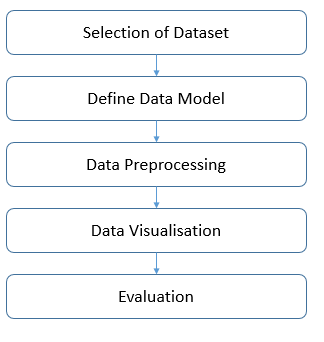
\includegraphics{Thesis_Goal.png}}
	
	\caption{Thesis Goals}
	\label{fig:labelOfMyFigure2}
\end{figure}
\subsection{Selection of Dataset}
In this thesis, we are looking for the high dimensional data set.There is no fixed threshold number of the dimension what can be termed as high but while we look for the data set we considered from visualisation perspective and ensure data set are high dimensional. If required we can convert the batch data to streaming data using any kind of state on art tool.
\subsection{Define Data Model}
The main difference between static data and streaming data is in static data we can save data into the disk and access that whenever we need that for any purpose but in streaming data the situation is not the same. In streaming data hence velocity of the data is huge so we can not save the data rather we need to do operations with the flow of data. Sliding window structure means we will divide the data in a block and only have access for once; there is no scope of viewing the data for the second time. The block can be done based on the time interval.
\subsection{Data Preprocessing}
Data preprocessing includes a lot of steps to be done before using the data. We will only focus on dimensionality reduction in this thesis and this is the core part of the thesis. There are many algorithms has been developed by researchers regarding Linear Discriminant Analysis and all of them either use the scatter matrix or QR decomposition under the big picture. Recently, one algorithm use Cholesky-decomposition to implement Linear Discriminant Analysis which is comparatively faster than others in theory but there is no open source of that code. Moreover, the algorithm is used for batch data set in an incremental way but we will directly imply the algorithm on stream data.
\subsection{Visualization}
Visualization is the beginning of the output section of the thesis.There are many state-on-art visualization techniques for visualize high dimensional data. We will visualize the output of the framework through one of the common procedure known as Heatmap.
\subsection{Evaluation}
There are basically two ways to evaluate the system. One is known as the quantitative evaluation and the other is qualitative evaluation. In Quantitative evaluation we define the metrics for example calculating the entropy or the matrix reordering quantitatively. Qualitative evaluation is the evaluation for example after showing the visualization by deciding which one is more informative. This can be done by doing user studies or selecting streaming data from different fields.\\\\
In our thesis we will follow the qualitative evaluation part by calculating different kind of matrices after getting the reduced dimensional data.\\\\
The remaining part of this paper is organized in the following manner: Section 2 will decribe the related work about dimensionality reduction, it will be followed by the solution of the thesis. Section 4 is for the evaluation and last section is the timeplan of the thesis. 


%\section{Figures}

%Use vector graphics wherever possible and avoid bitmap images. Do not
%use JPG at all (they are often blurred because of the compression). If
%you have to include a bitmap graphics, use the PNG format. If you have
%to use a JPG (as in the case for the logos on the title page), make sure
%that these are images with high resolution and high quality.
%\pdfcomment{pdfcomment is a useful package to put annotations like this one into the text.}

%The preferred way to create a PDF image to be used in LaTeX is the following:
%\begin{enumerate}
%\item Do the image with your favorite graphics program (Powerpoint works well for many cases).
%\item Print/Save the image as a PDF file (Acrobat Professional might be required, but
%there also Open Source solutions, e.g. FreePDF)
%\item Crop the image file and remove white margins.
%\item Include it in LaTeX as in this example.
%\end{enumerate}

%How to refer to images:
%Figure \ref{fig:labelOfFigure1} shows something from \cite{AfratiPODS2002}
%whereas figure \ref{fig:labelOfNextFigure} is about \cite{LenzeriniPODS2002}.

%If your image is not your own and taken from another source, cite the source
%also in the caption.

% priority where to place the figure: here, top, bottom, page
%\begin{figure}[htbp]
  % center the image.
 % \centering

  % include a png file. Adapt size to 0.5 * textwidth and retain aspect ratio (!)
 % \resizebox{\textwidth}{!}{
\includegraphics{Figure1.png}}

 % \caption{The text under the figure \cite{AfratiPODS2002}}
 % \label{fig:labelOfFigure1}
%\end{figure}


%\begin{figure}[htbp]
  %\centering
  % Include a pdf file but make it a little smaller than the textwidth
 % 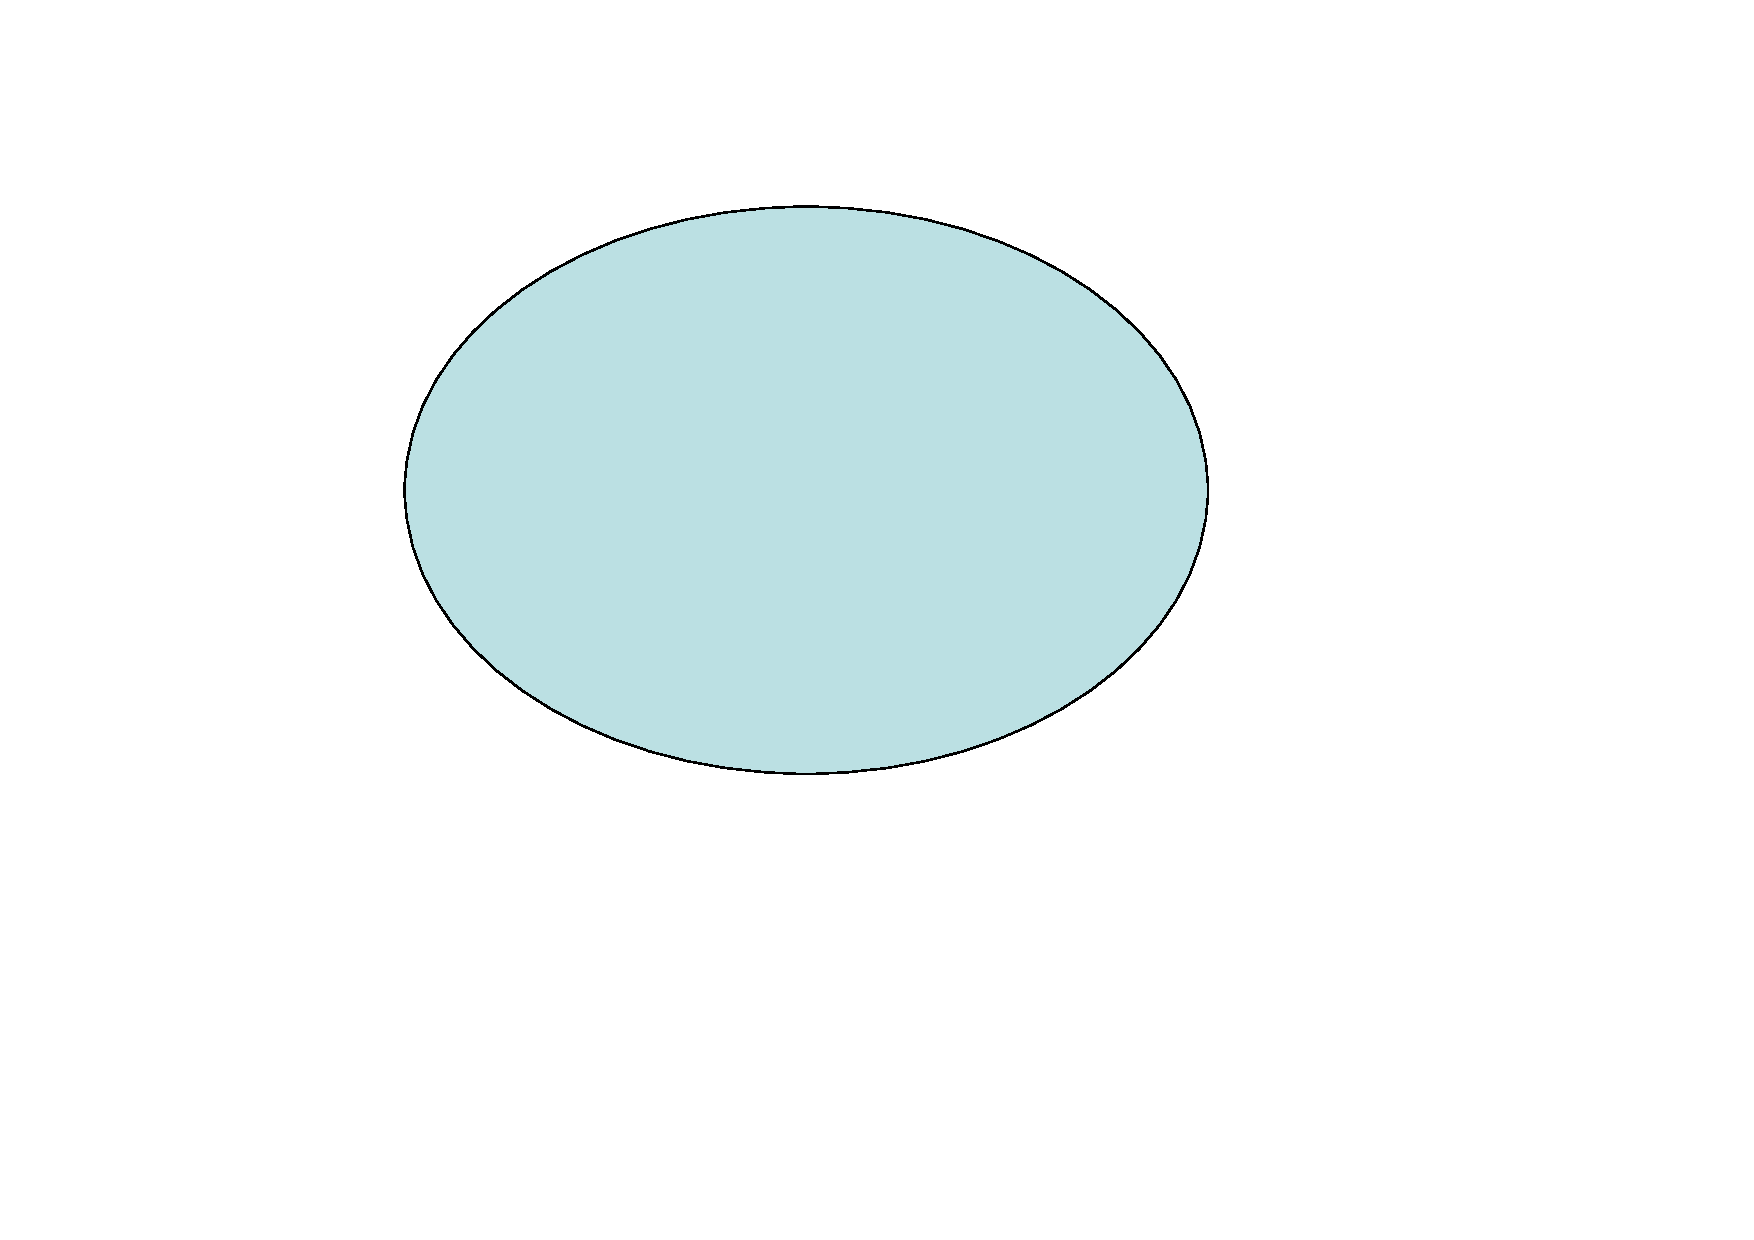
\includegraphics[width=0.5\textwidth]{Figure2.pdf}
  % Use EPS if you cannot create PDF files
  % (See http://www.wmf2eps.de.vu/ for creating eps files from powerpoint figures)
 % \caption{Another text under this figure \cite{LenzeriniPODS2002}}
 % \label{fig:labelOfNextFigure}
%\end{figure}



\chapter{Related Work}
\label{cha:relwork}

\begin{itemize}
\item Which similar/related works have been carried out?
\item If applicable: structuring of related work is good (e.g., if you have multiple related fields)
\item What is deficient in these works and what do they lack?
\item Compare the existing approaches in a table (different approaches in rows, features/requirements in columns)
and give a final discussion why a new approach (your thesis) is necessary
\end{itemize}



\section{Section 1}


The Chair of Computer Science 5 - Information Systems works on the formal
analysis, prototypical development, and practical testing of meta-information
systems. These systems are used to document and coordinate the distributed
design, integration, and evolution of database-centered applications in computer
science. Our research topics include Engineering Information Systems, Metadata
in Community Information Systems, Mobile Applications and Services, Database and
Meta-Database Technology, Technology Enhanced Learning and Model Management.

Informatik 5 is headed by Prof. Dr. M. Jarke who is also head of the Fraunhofer
Institute for Applied Information Technology (FIT). Prof. Jarke is founder
director of the Bonn-Aachen International Graduate Center for Information
Technology (B-IT). Affiliated to Informatik 5 are the teaching and research
areas for Knowledge-based Systems/Cognitive Robotics (Prof. Gerhard Lakemeyer,
Ph.D.), Visual Knowledge Management/Life Science Informatics (Prof. Dr. Thomas
Berlage), Cooperation Systems/CSCW (Prof. Wolfgang Prinz, Ph.D.) and Media
Informatics/Media Processes (Prof. Dr. Thomas Rose).


\section{Section 2}


The Chair of Computer Science 5 - Information Systems works on the formal
analysis, prototypical development, and practical testing of meta-information
systems. These systems are used to document and coordinate the distributed
design, integration, and evolution of database-centered applications in computer
science. Our research topics include Engineering Information Systems, Metadata
in Community Information Systems, Mobile Applications and Services, Database and
Meta-Database Technology, Technology Enhanced Learning and Model Management.

Informatik 5 is headed by Prof. Dr. M. Jarke who is also head of the Fraunhofer
Institute for Applied Information Technology (FIT). Prof. Jarke is founder
director of the Bonn-Aachen International Graduate Center for Information
Technology (B-IT). Affiliated to Informatik 5 are the teaching and research
areas for Knowledge-based Systems/Cognitive Robotics (Prof. Gerhard Lakemeyer,
Ph.D.), Visual Knowledge Management/Life Science Informatics (Prof. Dr. Thomas
Berlage), Cooperation Systems/CSCW (Prof. Wolfgang Prinz, Ph.D.) and Media
Informatics/Media Processes (Prof. Dr. Thomas Rose).


\section{Section 3}


The Chair of Computer Science 5 - Information Systems works on the formal
analysis, prototypical development, and practical testing of meta-information
systems. These systems are used to document and coordinate the distributed
design, integration, and evolution of database-centered applications in computer
science. Our research topics include Engineering Information Systems, Metadata
in Community Information Systems, Mobile Applications and Services, Database and
Meta-Database Technology, Technology Enhanced Learning and Model Management.

Informatik 5 is headed by Prof. Dr. M. Jarke who is also head of the Fraunhofer
Institute for Applied Information Technology (FIT). Prof. Jarke is founder
director of the Bonn-Aachen International Graduate Center for Information
Technology (B-IT). Affiliated to Informatik 5 are the teaching and research
areas for Knowledge-based Systems/Cognitive Robotics (Prof. Gerhard Lakemeyer,
Ph.D.), Visual Knowledge Management/Life Science Informatics (Prof. Dr. Thomas
Berlage), Cooperation Systems/CSCW (Prof. Wolfgang Prinz, Ph.D.) and Media
Informatics/Media Processes (Prof. Dr. Thomas Rose).


\section{Section 4}


The Chair of Computer Science 5 - Information Systems works on the formal
analysis, prototypical development, and practical testing of meta-information
systems. These systems are used to document and coordinate the distributed
design, integration, and evolution of database-centered applications in computer
science. Our research topics include Engineering Information Systems, Metadata
in Community Information Systems, Mobile Applications and Services, Database and
Meta-Database Technology, Technology Enhanced Learning and Model Management.

Informatik 5 is headed by Prof. Dr. M. Jarke who is also head of the Fraunhofer
Institute for Applied Information Technology (FIT). Prof. Jarke is founder
director of the Bonn-Aachen International Graduate Center for Information
Technology (B-IT). Affiliated to Informatik 5 are the teaching and research
areas for Knowledge-based Systems/Cognitive Robotics (Prof. Gerhard Lakemeyer,
Ph.D.), Visual Knowledge Management/Life Science Informatics (Prof. Dr. Thomas
Berlage), Cooperation Systems/CSCW (Prof. Wolfgang Prinz, Ph.D.) and Media
Informatics/Media Processes (Prof. Dr. Thomas Rose).


\section{Section 5}


The Chair of Computer Science 5 - Information Systems works on the formal
analysis, prototypical development, and practical testing of meta-information
systems. These systems are used to document and coordinate the distributed
design, integration, and evolution of database-centered applications in computer
science. Our research topics include Engineering Information Systems, Metadata
in Community Information Systems, Mobile Applications and Services, Database and
Meta-Database Technology, Technology Enhanced Learning and Model Management.

Informatik 5 is headed by Prof. Dr. M. Jarke who is also head of the Fraunhofer
Institute for Applied Information Technology (FIT). Prof. Jarke is founder
director of the Bonn-Aachen International Graduate Center for Information
Technology (B-IT). Affiliated to Informatik 5 are the teaching and research
areas for Knowledge-based Systems/Cognitive Robotics (Prof. Gerhard Lakemeyer,
Ph.D.), Visual Knowledge Management/Life Science Informatics (Prof. Dr. Thomas
Berlage), Cooperation Systems/CSCW (Prof. Wolfgang Prinz, Ph.D.) and Media
Informatics/Media Processes (Prof. Dr. Thomas Rose).


\section{Section 6}


The Chair of Computer Science 5 - Information Systems works on the formal
analysis, prototypical development, and practical testing of meta-information
systems. These systems are used to document and coordinate the distributed
design, integration, and evolution of database-centered applications in computer
science. Our research topics include Engineering Information Systems, Metadata
in Community Information Systems, Mobile Applications and Services, Database and
Meta-Database Technology, Technology Enhanced Learning and Model Management.

Informatik 5 is headed by Prof. Dr. M. Jarke who is also head of the Fraunhofer
Institute for Applied Information Technology (FIT). Prof. Jarke is founder
director of the Bonn-Aachen International Graduate Center for Information
Technology (B-IT). Affiliated to Informatik 5 are the teaching and research
areas for Knowledge-based Systems/Cognitive Robotics (Prof. Gerhard Lakemeyer,
Ph.D.), Visual Knowledge Management/Life Science Informatics (Prof. Dr. Thomas
Berlage), Cooperation Systems/CSCW (Prof. Wolfgang Prinz, Ph.D.) and Media
Informatics/Media Processes (Prof. Dr. Thomas Rose).


\section{Section 7}


The Chair of Computer Science 5 - Information Systems works on the formal
analysis, prototypical development, and practical testing of meta-information
systems. These systems are used to document and coordinate the distributed
design, integration, and evolution of database-centered applications in computer
science. Our research topics include Engineering Information Systems, Metadata
in Community Information Systems, Mobile Applications and Services, Database and
Meta-Database Technology, Technology Enhanced Learning and Model Management.

Informatik 5 is headed by Prof. Dr. M. Jarke who is also head of the Fraunhofer
Institute for Applied Information Technology (FIT). Prof. Jarke is founder
director of the Bonn-Aachen International Graduate Center for Information
Technology (B-IT). Affiliated to Informatik 5 are the teaching and research
areas for Knowledge-based Systems/Cognitive Robotics (Prof. Gerhard Lakemeyer,
Ph.D.), Visual Knowledge Management/Life Science Informatics (Prof. Dr. Thomas
Berlage), Cooperation Systems/CSCW (Prof. Wolfgang Prinz, Ph.D.) and Media
Informatics/Media Processes (Prof. Dr. Thomas Rose).




\chapter{Solution}
\label{cha:solutioni}

%Give a (detailed) description of the approach:

%\begin{itemize}
%\item give reasons, why you decided for specific parts of the approach
%\item its also a good idea to compare with related work (because this
%		  approach did not work so well in \cite{conf/vldb/KenscheQXlYl07} the authors used..)
%\item In the proposal: a rough design (e.g., an architecture, algorithm) of the approach,
%		  clarifying what will be done by you and what is already there/is a ready-to-use part
%		  (e.g., a library, product you use). Give also some details about the technologies
%		  which you want to use in the thesis project.
%\item In the thesis: a conceptual description of your approach. Important: do not go into
%      implementation details at this stage. Give an overall picture (e.g., system architecture, data flow
%      diagram, sequence diagrams for an algorithm, etc.). Explain the main components of your solution
%      and give short description of any external or existing component which is used by your system.
%      Give conceptual models (e.g., EER diagrams) of your data structures.
%\item Important: describe the \emph{process} of getting to the final solution, do
%      not describe only the final solution. All design decisions are important (I preferred
%      X, because Y performs badly).
% \end{itemize}
At present due to the increment of mobile devices huge number of streaming data are being generated. Unfortunately, these datasets are not in an organised as it should be for the analysis. There are many null values in the dataset and the data are being high-dimensional as well. To analyse this kind of data we need to implement fast pre-processing steps to analyse those data sets. One of the important preprocessing technique is dimensionality reduction. 

An extensible framework to reduce the dimensions of streaming data with a concept of modularity of each component. To achieve this goal, framework is designed in such a way that each component act as a stand alone component but can be interacted with each other in a very convenient way. Moreover, the components are  plug-in and play designed architecture. Each component can be easily replaced or added more functionality through out the whole implementation phase when it is necessary.

In a broadshell, there are three modules of the whole framework which are listed below:
\begin{itemize}
	\item Data Set Load and Processing Module
	\item Dimensionality Reduction Module
	\item Visualization Module
\end{itemize}

Each module has its own responsibilty of the total framework. The task is divided in such a way so that the separation of concern principle exists. Each module is considered as a distinct section so that each section addresses a totally separate task. However, there are some interdependency of executing the order of component which will be addressed into the implementaiton part.

The architecture of the framework is the multitier architecture. From software engineering perspective in multitier architecture\footnote{\url{https://en.wikipedia.org/wiki/Multitier_architecture}} client-server are involved where presentation, application processing and data management functions are physically separated.
\begin{enumerate}
	\item Persistence Layer
	\item Business Layer
	\item Access Layer
	\item Presentation Layer
\end{enumerate}

According to the defintion from software perspective,  operation with the all data 

\begin{figure}[htbp]
	% center the image.
	\centering
	
	% include a png file. Adapt size to 0.5 * textwidth and retain aspect ratio (!)
	\resizebox{\textwidth}{!}{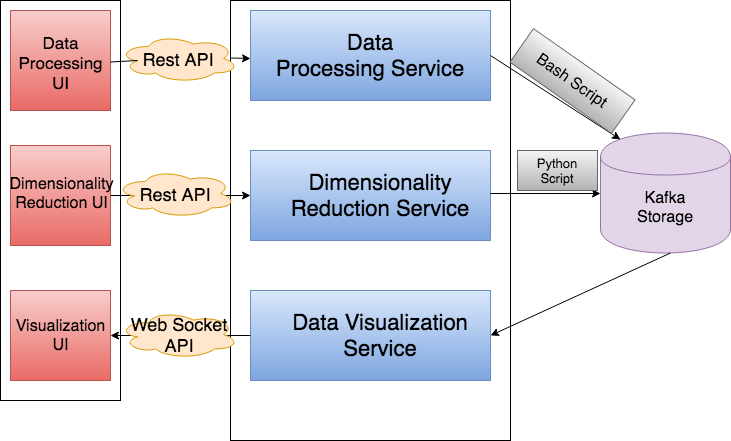
\includegraphics{architecture_thesisReport.png}}
	
	\caption{Architecture/ Design for the Extensible Framework}
	\label{fig:labelOfThesisFlowChart}
\end{figure}

In this section, I will describe the solution approach of reducing the high dimensional streaming data to low dimensional streaming data.\\\\
The following figure \ref{fig:labelOfThesisFlowChart} contains the general process model of our Framework.
\begin{figure}[htbp]
	% center the image.
	\centering
	
	% include a png file. Adapt size to 0.5 * textwidth and retain aspect ratio (!)
	\resizebox{\textwidth}{!}{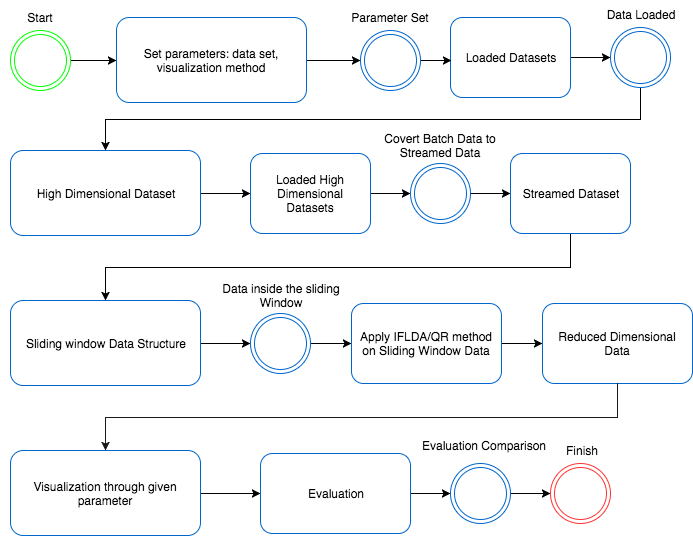
\includegraphics{Thesis_Flow_chart.png}}
	
	\caption{Dimensionality Reduction Framework of Streamed Data}
	\label{fig:labelOfThesisFlowChart}
\end{figure}
\subsection{Selection of Data Sets}
The framework will be flexible for both the online available streaming API to consider as a data source and also have the ability to upload the static data. Hence we are considering the streaming data it will be good if the chosen data domain have some impacts on the change of the data with the passage of the time.\\\\
If the chosen data set is not the streaming data then the framework will be capable enough to convert the static data to the streaming data using any available free state-on-art tools.
\subsection{Define Data Model}
The main characteristics of the streaming data that the data comes continuously with an unbounded structure and pattern as time progresses. For this reason, to handle the streaming data there should be some mechanism to hold the data for a minimum period of time and within that time all necessary work related with the data should be done then the data is thrown off. One of the common mechanism to handle those data is known as sliding window approach. Here the window is defined based on the time like in particular interval for example in each 500 ms the data comes are considered one window. The window will be moved after each fixed period of time and that's the reason it is known as sliding window approach. Our framework will be capable of considering the streaming data in a sliding window basis.
\subsection{IFLDA/QR algorithm}
As previously mentioned we will implement the IFLDA/QR algorithm. At the first window, we will implement the FLDA algorithm to calculate the centroid matrix and implement the Cholesky Decomposition of the centroid matrix. The output of this mechanism is the optimal transformation matrix.\\\\
From second window and so on we will implement the algorithm of the insertion of the chunk data. Here as an input of the process we will consider labeled new samples and also the novel class. Here the centroid matrix for an existing class will be updated as well as the new centroid of the new cluster will be calculated.In following figure \ref{fig:labelOfChunkData} the whole process is shown step by step wise.
\begin{figure}[htbp]
	% center the image.
	\centering
	
	% include a png file. Adapt size to 0.5 * textwidth and retain aspect ratio (!)
	\resizebox{\textwidth}{!}{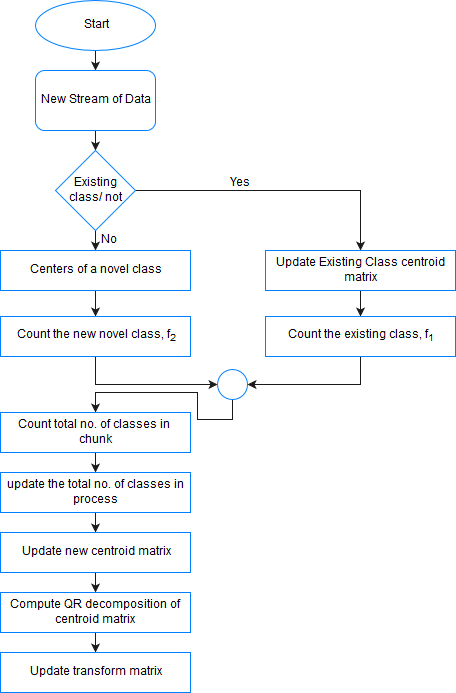
\includegraphics{chunk_data_process.png}}
	
	\caption{Process of Handling Stream Data}
	\label{fig:labelOfChunkData}
\end{figure}
\subsection{Data Visualization}
The final outcome of the framework will be the visualization. In visualization, we will see the inner relationship of the data. In this case, visualization will not be only used for the communication to the end user but also it will reveal the inner meanings of the data for example, the pattern of the data, the relationship among the features and many more. The visulaisation tool we used here will be the Heatmap, one of the most used visualization tool for high dimensional data.

\subsection{Design Framework}
In this section, we will describe the design of the framework in details. The framework should have ability to  extend for further implementation if needed. Moreover, the component should be reusable. The framework will also have the separation of concerns by allocating tasks to different layers.\\\\
The whole design Framework has four layers: 
\begin{enumerate}
	\item Persistence Layer
	\item Business Layer
	\item Access Layer
	\item Presentation Layer
\end{enumerate}
Each layer will be associated individual category of tasks. In Persistence layer the data will be saved and used for the tasks involved with data. The Business layer is responsible for doing all back end task for the framework. Through Access layer, Business layer and Presentation layer will communicate with each other where Presentation layer is responsible to present the data and take input from the user.\\\\   
This whole section will be further divided into three subsections. We will describe the requirements list at the beginning then the overall design of the framework and last but not the least the sequence diagram of the framework.
\subsubsection{List of Requirements }
The whole requirements for the framework will be described in this section. The framework should be adaptable enough to response based on the user input. Till now, the framework should meet the following requirements. 
\begin{enumerate}
	\item User can select data type from stream data or batch Data
	\item User can choose data set from available dataset
	\item User can add new dataset to the specified place by uploading to the framework
	\item User will get the reduced dimensional data for given input data
	\item User can select the time interval for observing the visualization
	\item User can select the required evaluation criteria from the evaluation list and show the evaluation information.
\end{enumerate}
\subsubsection{Architecture Diagram} 
In this section we will present the architecture diagram of the framework.  As mentioned, the architecture is divided into four sections and each section has separate components for the different concerns. In fig \ref{fig:labelOfFrameworkArchitecture}, each section is defined with the individual components. Each component is responsible for fixed set of requirements. Each layer has a bi-directional communication where one layer is communicated with others.
\begin{figure}[htbp]
	% center the image.
	\centering
	
	% include a png file. Adapt size to 0.5 * textwidth and retain aspect ratio (!)
	\resizebox{\textwidth}{!}{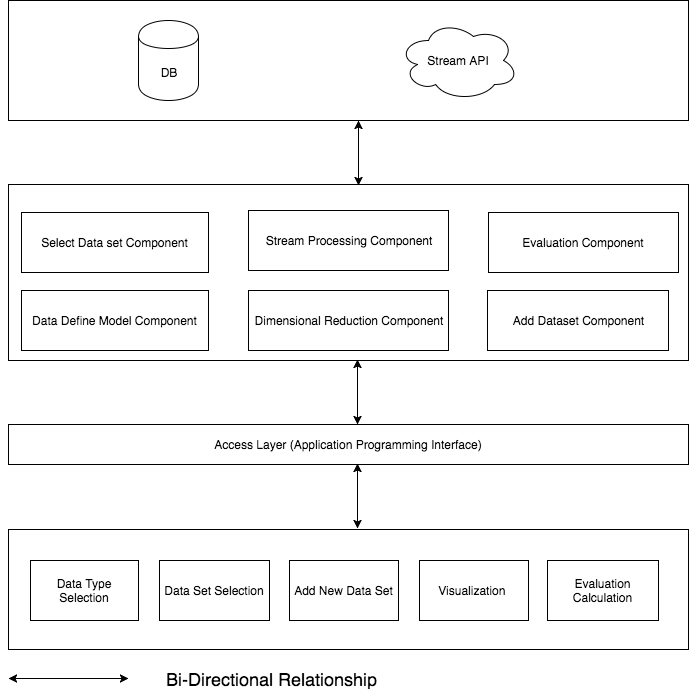
\includegraphics{DRFW_Visualization_Architecture.png}}
	
	\caption{Framework Architecture}
	\label{fig:labelOfFrameworkArchitecture}
\end{figure}
Based on the requirements a particular set of component is assigned for a fixed task. In Persistence layer, all information of the data is stored and ability to perform both read and write operation. There are in total five components in Business layer for performing all the requirements. The Access layer is all used for the communication using Application Programming Interface. There are five different ways for the user to communicate with the framework.
In Presentation layer, the user will send the parameter data to the Business layer \& receive data after the process done. In Business layer for implementing business logic it will communicate with the Persistence layer and send data to the front end. In addition, the business layer will also do the mathematical calculation for presenting evaluation information to the presentation layer. \\\\
In Presentation layer, user can give three inputs for showing the intended output: Select Data type, Dataset, Time interval selection, Select evaluation parameter. For adding new dataset user can upload to the framework. The details requirement list for the Presentaiton layer is listed below:
\begin{itemize}
	\item Select Data type: User can select either Stream Data or Batch Data
	\item Select Dataset: User can choose data set from Available Dataset
	\item Add new Dataset: User can add new dataset to the specified place by uploading
	\item Show Visualization based on given time interval: Here, user will select at what interval of time user wants to visualize and be able to watch visualization
	\item Evaluation Information: User can show the evaluation information for example information loss will be shown in continuous fashion
\end{itemize}
From Presentation layer the framework will access the Business layer through Access layer. The framework will have few Application Programming Interface associated with each task. In Business layer, the framework will implement the business logic of the framework. The details requirement list for the Business layer is listed below:
\begin{itemize}
	\item Save Datasets to Database: Framework should save the dataset that user gives to the Presentation layer and give feedback in both accept state or rejection state. The dataset should be available from that point on wards in the framework if accepted.
	\item List of available Datasets: If user selects the Batch data then framework should send all the  available datasets to the user for selection.
	\item Stream Processing: The framework should be able to detect whether selected type is batch or stream. If Selected type is stream than this component should not do any further tasks otherwise the framework will convert the static data to the stream data
	\item Data Define Model: After selection of the data the framework should capture the data for the fixed time window and apply the dimensionality reduction on that window.
	\item Dimensionality Reduction: Framework should be able to reduce the dimensions of the input dataset.
\end{itemize}

\subsubsection{Sequence Diagram}
In this section, the corresponding sequence of each requirement is described in details like how the request/ response is communicated from each layer through out the framework and also start or finishing time of any requirement. In fig \ref{fig:labelOfSequenceDiagram} the whole process is shown in details.
\begin{figure}[htbp]
	% center the image.
	\centering
	
	% include a png file. Adapt size to 0.5 * textwidth and retain aspect ratio (!)
	\resizebox{\textwidth}{!}{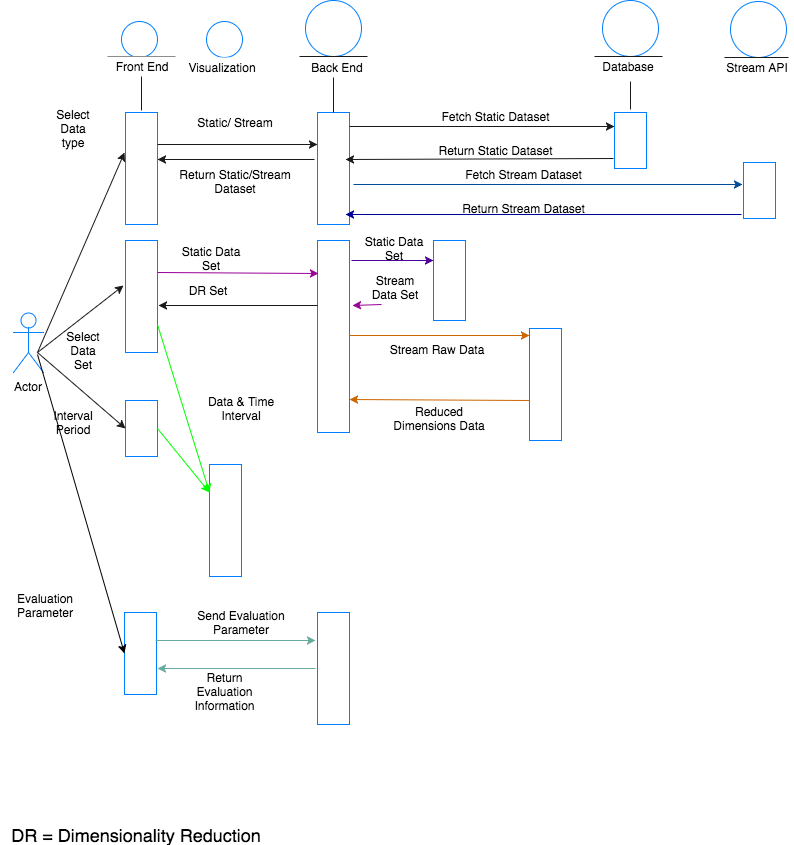
\includegraphics{Sequence_Diagram.png}}
	
	\caption{Sequence Diagram}
	\label{fig:labelOfSequenceDiagram}
\end{figure}
The total sequence diagram is explained in step wise one after another.
\paragraph{Selection of Data Type: }
User will select the data type and this value will be send to the backend. The value will be saved and send to "Select Data set" component . From backend, it will communicate to the database and receive the available data set. If the type is stream then it will directly communicate with the cloud and collect the available datasets from that stream. The dataset will be either a set of the static data or a set of streaming Application Program Interface.
\paragraph{Show Visualization based on time interval:}
User will select the time to define the frame of each window. This input will be required to the Business layer to "Data Define Model" component. User will also select time interval to see the visualization after a certain interval. For example, if the given interval value is 5 then user will see the visualisation after 5 window respectively.  
\paragraph{Selection of Data Set:}
User will select the data set from the available data set from the previous step . If the selected data set is "Batch" data set then from persistence layer it will go the "Stream Processing" component. The main task of this component is to convert static to stream data. If the type is "Stream" then this component has nothing to do other than sending void. This stream data will be used for further process.\\\\
Now the stream data along with the window frame size will go to the "Dimensional Reduction" component. This component is the heart of the framework. This component will be responsible to reduce the dimensions by implementing the algorithm and send back to Persistence layer. Based on the given interval value, the persistence layer will show the visualization in segment "Visualization" of the Persistence layer.
\paragraph{Evaluation Information:}
Here the list of all possible evaluation criteria will be given in "Evaluation" of the presentation layer. From the given value it will communicate with the "Evaluation" component of the persistence layer and show the value to the user.
\paragraph{Add new Dataset:}
User will also be able to add new data set or a cloud Stream API. From Presentation layer with the given data set it will go the Business layer. From there Business layer will communicate  with the Persistence layer and save the value. The datset or API should be available from that time on if required.



% Evaluation in a separate chapter or as subsection of solution approach
\chapter{Evaluation}
\label{cha:eval}

%\begin{itemize}
%\item In the proposal: describe the data sets and measures which you plan
%      to use in the evaluation. Make sure that the resources (data, users, etc.)
%      which are required for the evaluation are really available.
%\item In the thesis: describe the data sets and measures which you have used.
%      Give the results in form of diagrams (e.g., Excel or Gnuplot). Discuss
%      different variants of your solutions and different parameter settings.
%     If available, compare your results with an existing approach. Important:
%      Also negative results are results: ``The approach did not work for this
%      data set because ...'' This is important information, because nobody wants
%      to do again the same experiments as you already did. In case of performance
%      numbers, give a detailed description of the hardware which was used to do
%      the experiments. Discuss the results (what is good, what is bad).
%\end{itemize}
We will evaluate the visualization of framework through different ways. The evaluation will help us to measure the quality of our framework. The rate of data arrival is very high in stream data. Therefore it's a big challenge for the framework to adopt itself with the flow of data. Secondly, the presence of data will be for a limited time and there is no chance of data availability for the second time so it's also a challenge for the framework to visualize the correct result just by using once. Last but not the least, data will be unpredictable and unbounded in structure therefore framework need to be stable from that perspective as well.\\\\
As previously mentioned, evaluation can be done in two different ways: Quantitative evaluation, Qualitative evaluation. Here, we will focus more on the Qualitative evaluation through comparative methodology. The first comparison will be regarding the studying of effect of data reduction through visualization. Our framework will be able to give the visualization without applying the data reduction framework and after applying data reduction. Hence, information loss is must while applying data reduction; we will calculate the Entropy matrix for calculating the amount of information loss.\\\\
Our second evaluation will be done regarding the comparison of performance between using incremental data and also the streaming data. Our framework will be flexible to use data in both ways. Through this, we can show the effect of interrupting continuous flow of data to the visualization. To calculate this we will use the Earth-Mover distance matrix for that. \\\\
Our framework should be scalable enough to adopt as the number of dimensions increase. The framework will be tested with the excel of dimensions. \\\\
For evaluation, the framework will be tested with the expert user from domain field. We will observe how the expert user is gaining the knowledge or communicated through out the visualization and how they understand the inner meaning of the visualization. The framework will also be tested by giving a new data set from the user and see the performance of the framework.\\\\

The following list contains the evaluation criteria of our framework.
\begin{enumerate}
	\item Studying the effect of data reduction on the visualization quality. 
	\item Comparison of performance of the algorithm between using incremental data and streaming data
	\item Scalability of the Framework with the increase of dimensions.
	\item Calculate the evaluation matrix: Entropy calculation, Earth-Mover Distance.
\end{enumerate}

\chapter{Timeplan}
\label{cha:timeplan}

\begin{itemize}
\item Include a gantt chart here (do it with MS Visio or Excel),
it should have about 10 tasks clustered into about 4 groups:
literature study, design, implementation, evaluation.
\item Give a brief explanation of the timeplan.
\end{itemize}



% References
\bibliographystyle{apalike}
\bibliography{Bib}












\end{document}


